\subsection{Módulo de Procesos}\label{subsec:procesos}

El Módulo de Procesos constituye el núcleo operativo de la plataforma, dotando a los usuarios de las herramientas necesarias para la búsqueda, vinculación y gestión de los procesos judiciales de su interés. Su desarrollo abarca desde herramientas para la consulta manual y un panel de control centralizado, hasta capacidades de automatización mediante el monitoreo constante de expedientes. Todo esto involucró la creación de interfaces de usuario interactivas, la integración con servicios externos de información jurídica y la construcción de una sólida capa de comunicación con el \textit{backend} del sistema.

\subsubsection{Panel de Control Centralizado (Dashboard)}

Para ofrecer una experiencia de usuario eficiente y reducir la fricción operativa, se desarrolló una vista principal (\textit{Dashboard}) que actúa como el punto de entrada para el usuario autenticado. Esta interfaz fue diseñada bajo un enfoque de modularidad, componiéndose de diversas tarjetas y \textit{widgets} interactivos que consolidan la información más relevante de la cuenta. A través de este panel, el usuario obtiene una visión panorámica e inmediata de sus estadísticas generales, el estado de sus planes activos y el acceso directo a sus procesos judiciales más recientes, facilitando la toma de decisiones y permitiendo ejecutar acciones rápidas sin la necesidad de navegar profundamente por las distintas secciones de la plataforma. La \autoref{fig:dashboard-procesos} muestra el \textit{dashboard} principal con sus componentes de resumen, estadísticas y accesos directos organizados en una cuadrícula adaptativa.

\newcommand\dashboardProcesosCaption{\textit{Dashboard} principal del módulo de procesos con estadísticas y accesos directos al usuario. \hspace{1em}}
\begin{figure}[H]
  \centering
  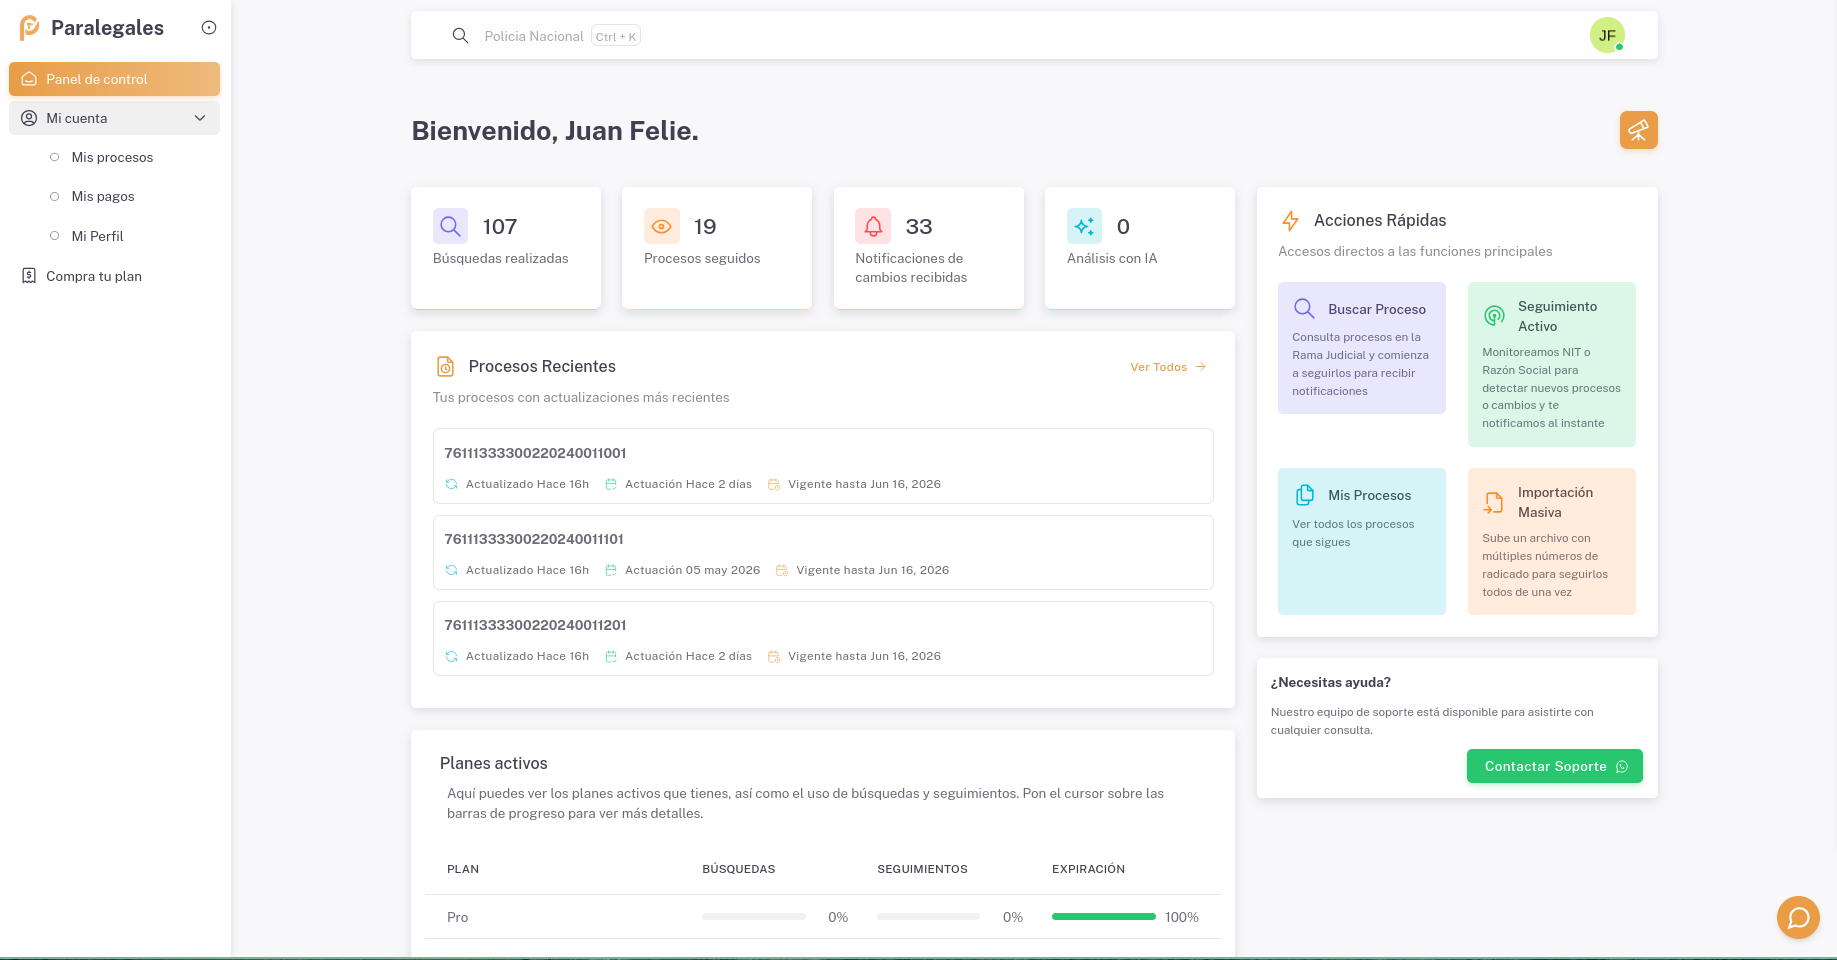
\includegraphics[width=1\textwidth]{img/figures/fig23-dashboard-procesos.png}
  \caption[\dashboardProcesosCaption]{\dashboardProcesosCaption Fuente: Elaboración propia.}
  \label{fig:dashboard-procesos}
\end{figure}

\subsubsection{Búsqueda de Procesos e Integración con la Rama Judicial}

Uno de los requerimientos más críticos de la plataforma fue proveer un motor de búsqueda que permitiera consultar procesos directamente desde las bases de datos de la Rama Judicial. Dado que la entidad proporciona un portal público pero carece de una API documentada y orientada a desarrolladores, se llevó a cabo un proceso de ingeniería inversa que consistió en interceptar, analizar y mapear el tráfico de red generado por el portal oficial durante consultas legítimas. A través de este análisis, se identificaron los distintos \textit{endpoints} utilizados por la entidad y la estructura de los \textit{payloads} requeridos, abarcando desde las consultas de parametrización (departamentos, ciudades, especialidades y entidades) hasta las búsquedas directas por código de radicado o nombre del implicado.

Para la integración a nivel de software, se diseñó una arquitectura de \textit{proxy} en el servidor de la aplicación. En lugar de que el \textit{frontend} realizara las peticiones directamente a los servidores gubernamentales, estas se encapsularon en una capa de servicios intermediarios dentro del BFF. Esta decisión arquitectónica aportó múltiples beneficios: permitió superar las restricciones de políticas de mismo origen (CORS), estandarizó los esquemas de respuesta hacia las vistas de la aplicación, y habilitó la incorporación de capas de observabilidad, manejo de errores centralizado y generación de \textit{logs} de auditoría. En el \textit{frontend}, las vistas de resultados consumen esta API interna de forma segura y estructurada, presentando la información judicial al usuario de manera clara y eficiente.

La \autoref{fig:filtros-busqueda-procesos} expone el formulario de búsqueda avanzada, donde el usuario puede combinar múltiples criterios de filtrado —como departamento, ciudad, especialidad y entidad— para acotar el universo de expedientes consultados. La \autoref{fig:resultados-busqueda} ilustra la vista de resultados que despliega la lista de procesos encontrados, con la información relevante de cada expediente organizada de forma tabular y con indicadores de estado claramente diferenciados.

\newcommand\filtrosBusquedaProcesosCaption{Formulario de búsqueda avanzada de procesos judiciales con filtros combinables. \hspace{1em}}
\begin{figure}[H]
  \centering
  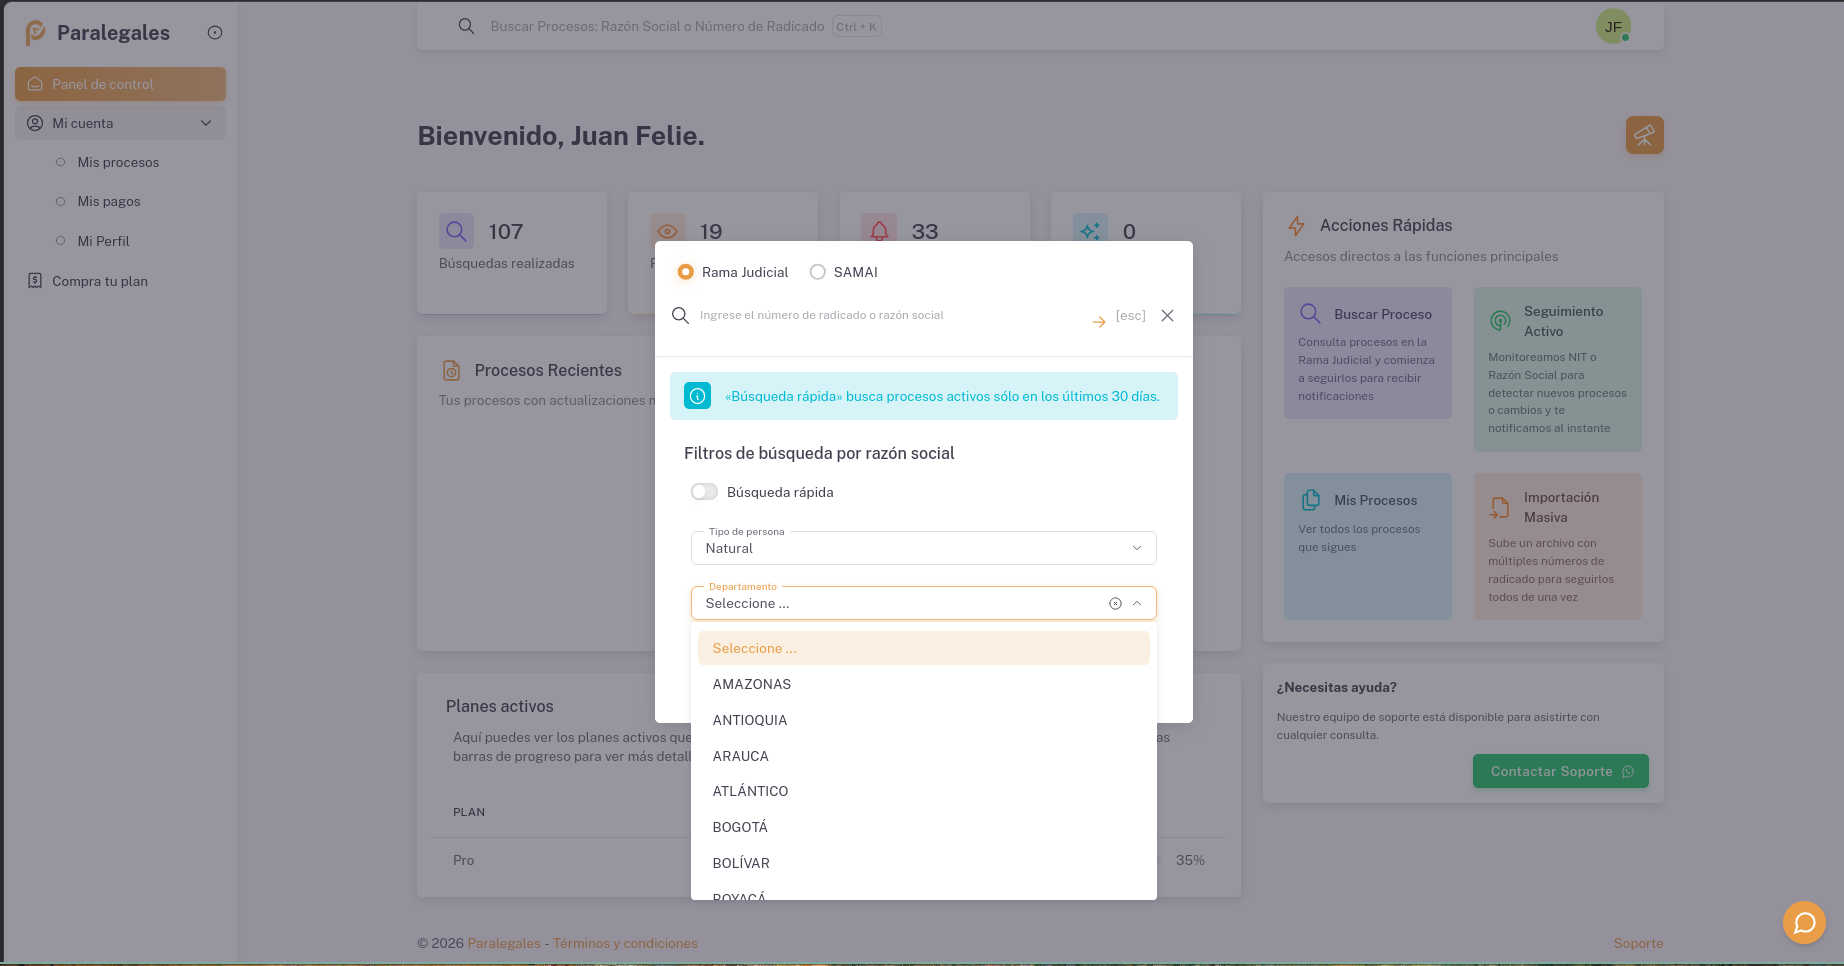
\includegraphics[width=1\textwidth]{img/figures/fig24-filtros-busquedas-procesos.png}
  \caption[\filtrosBusquedaProcesosCaption]{\filtrosBusquedaProcesosCaption Fuente: Elaboración propia.}
  \label{fig:filtros-busqueda-procesos}
\end{figure}

\newcommand\resultadosBusquedaCaption{Vista de resultados de la búsqueda de procesos judiciales en la Rama Judicial. \hspace{1em}}
\begin{figure}[H]
  \centering
  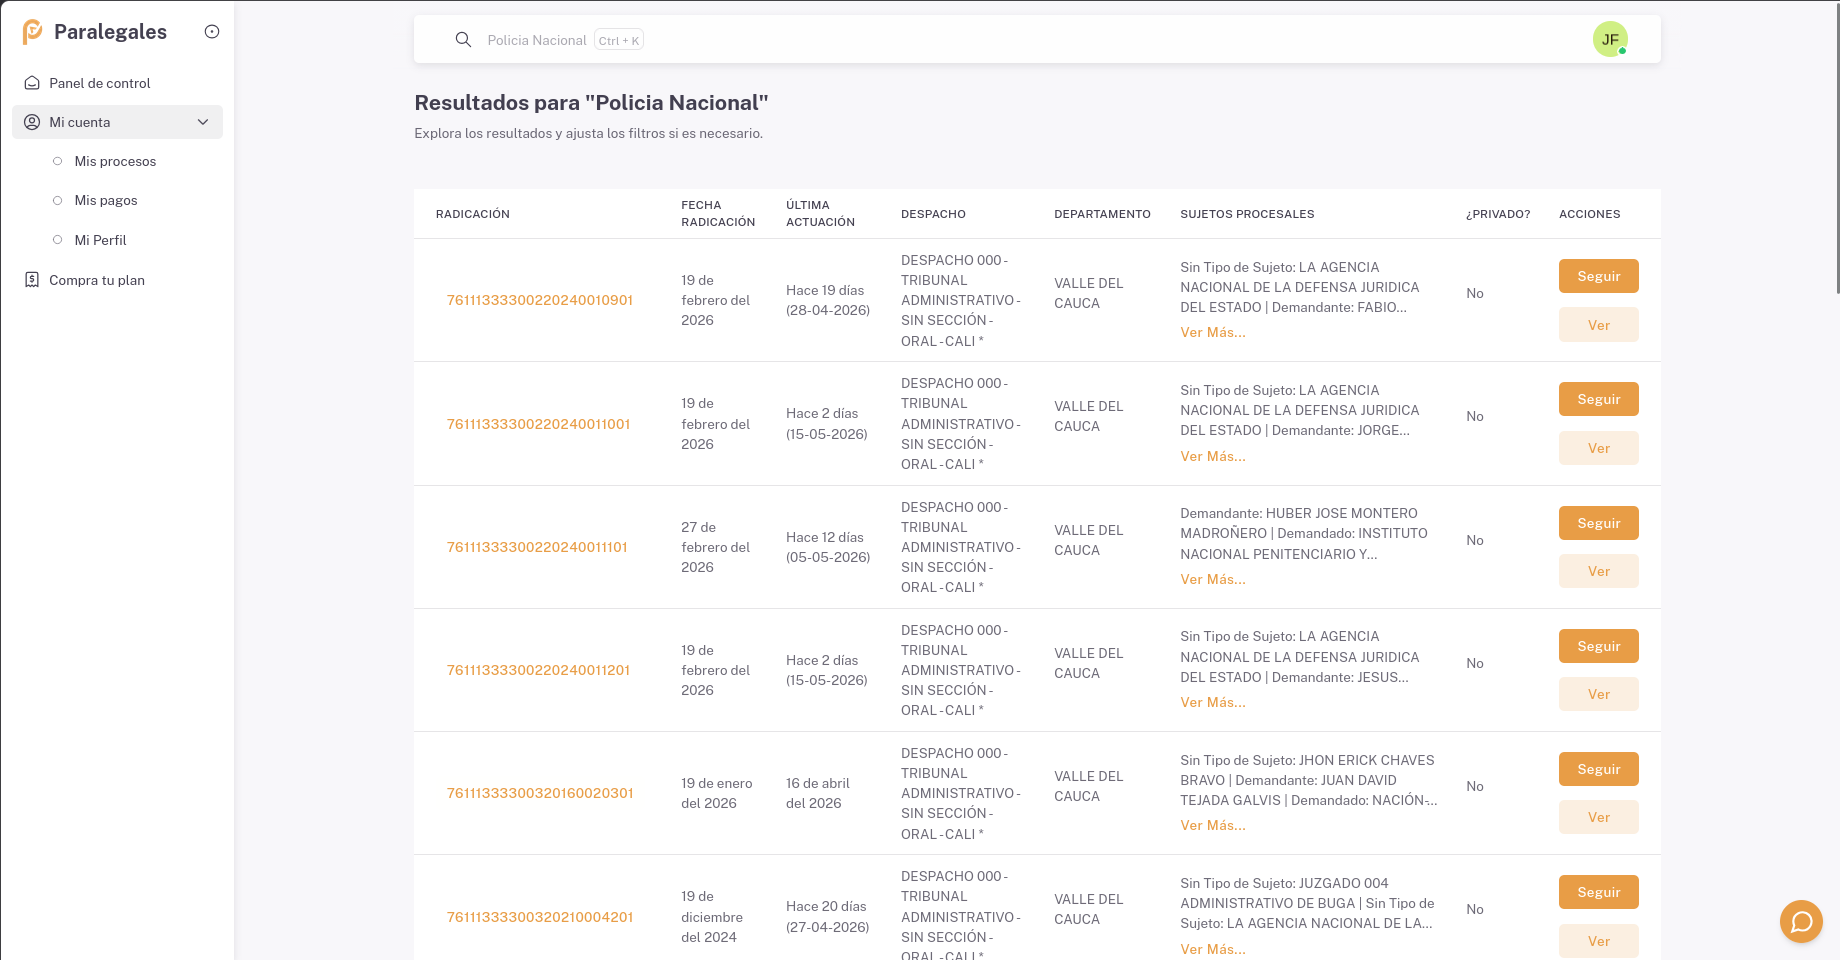
\includegraphics[width=1\textwidth]{img/figures/fig25-results-process.png}
  \caption[\resultadosBusquedaCaption]{\resultadosBusquedaCaption Fuente: Elaboración propia.}
  \label{fig:resultados-busqueda}
\end{figure}

\subsubsection{Seguimiento de Procesos}

Una vez localizado un proceso a través del motor de búsqueda, el sistema le brinda al usuario la capacidad de agregarlo a su portafolio personal para un monitoreo continuo. Esta funcionalidad de seguimiento (\textit{follow}) y cancelación del mismo (\textit{unfollow}) requirió un diseño cuidadoso para garantizar una experiencia reactiva e instantánea.

En el \textit{frontend}, la implementación separa estrictamente la capa de presentación de la lógica de negocio: se desarrollaron componentes visuales atómicos y reutilizables —como botones interactivos con estados de carga— cuya lógica de interacción fue abstraída mediante \textit{composables}. Estos encapsulan el manejo del estado local, la reactividad y las excepciones, invocando a su vez repositorios dedicados a la comunicación de red. La orquestación lógica de asociar o desvincular un proceso a un usuario fue delegada y centralizada en los servicios \textit{backend}, de modo que el \textit{frontend} solo emite la intención del usuario y reacciona al resultado actualizando la interfaz de forma instantánea. La \autoref{fig:follow-process} presenta el componente de acción de seguimiento integrado en la vista de resultados, donde el usuario puede vincular un expediente a su cuenta mediante una única interacción.

\newcommand\followProcessCaption{Componente de seguimiento de proceso judicial accesible desde la vista de resultados de búsqueda. \hspace{1em}}
\begin{figure}[H]
  \centering
  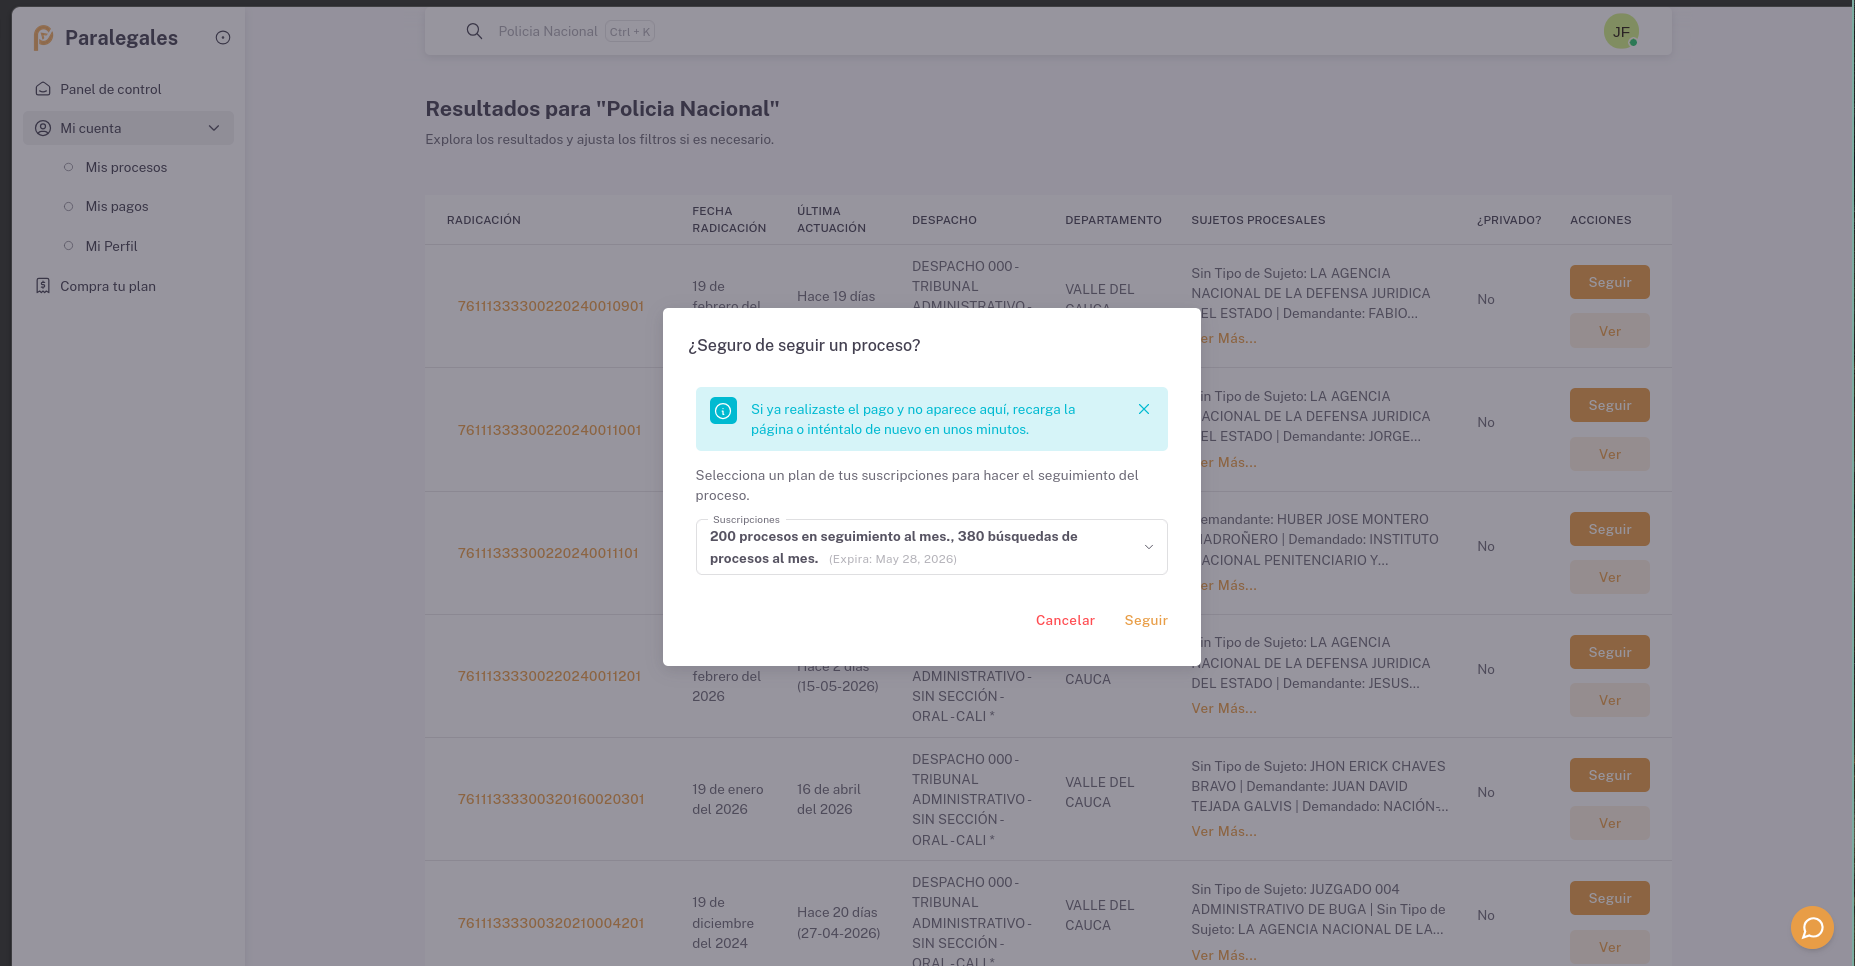
\includegraphics[width=1\textwidth]{img/figures/fig26-follow-process.png}
  \caption[\followProcessCaption]{\followProcessCaption Fuente: Elaboración propia.}
  \label{fig:follow-process}
\end{figure}

\subsubsection{Gestión y Visualización: Mis Procesos}

Para centralizar la información de cada usuario, se desarrolló la vista ``Mis Procesos'', que actúa como el panel de control personal del usuario, listando en un formato estructurado y amigable todos los procesos bajo seguimiento activo.

El diseño de esta vista se enfocó en la modularidad y el rendimiento. La interfaz recupera de manera asíncrona la lista de procesos vinculados al usuario autenticado a través de la interacción entre el cliente y el \textit{backend}. El componente es altamente reactivo: si el usuario decide cancelar el seguimiento de un proceso desde este panel, el sistema invoca la abstracción de seguimiento descrita anteriormente y el proceso se elimina de la vista en tiempo real, sin requerir recargas de página, ofreciendo una experiencia ininterrumpida. Como se aprecia en la \autoref{fig:my-processes-view}, la vista organiza los expedientes en tarjetas con información resumida —radicado, entidad, estado y fecha de última actuación—, permitiendo al usuario identificar rápidamente los casos que requieren su atención.

\newcommand\myProcessesViewCaption{Vista ``Mis Procesos'' con la lista de expedientes bajo seguimiento activo del usuario. \hspace{1em}}
\begin{figure}[H]
  \centering
  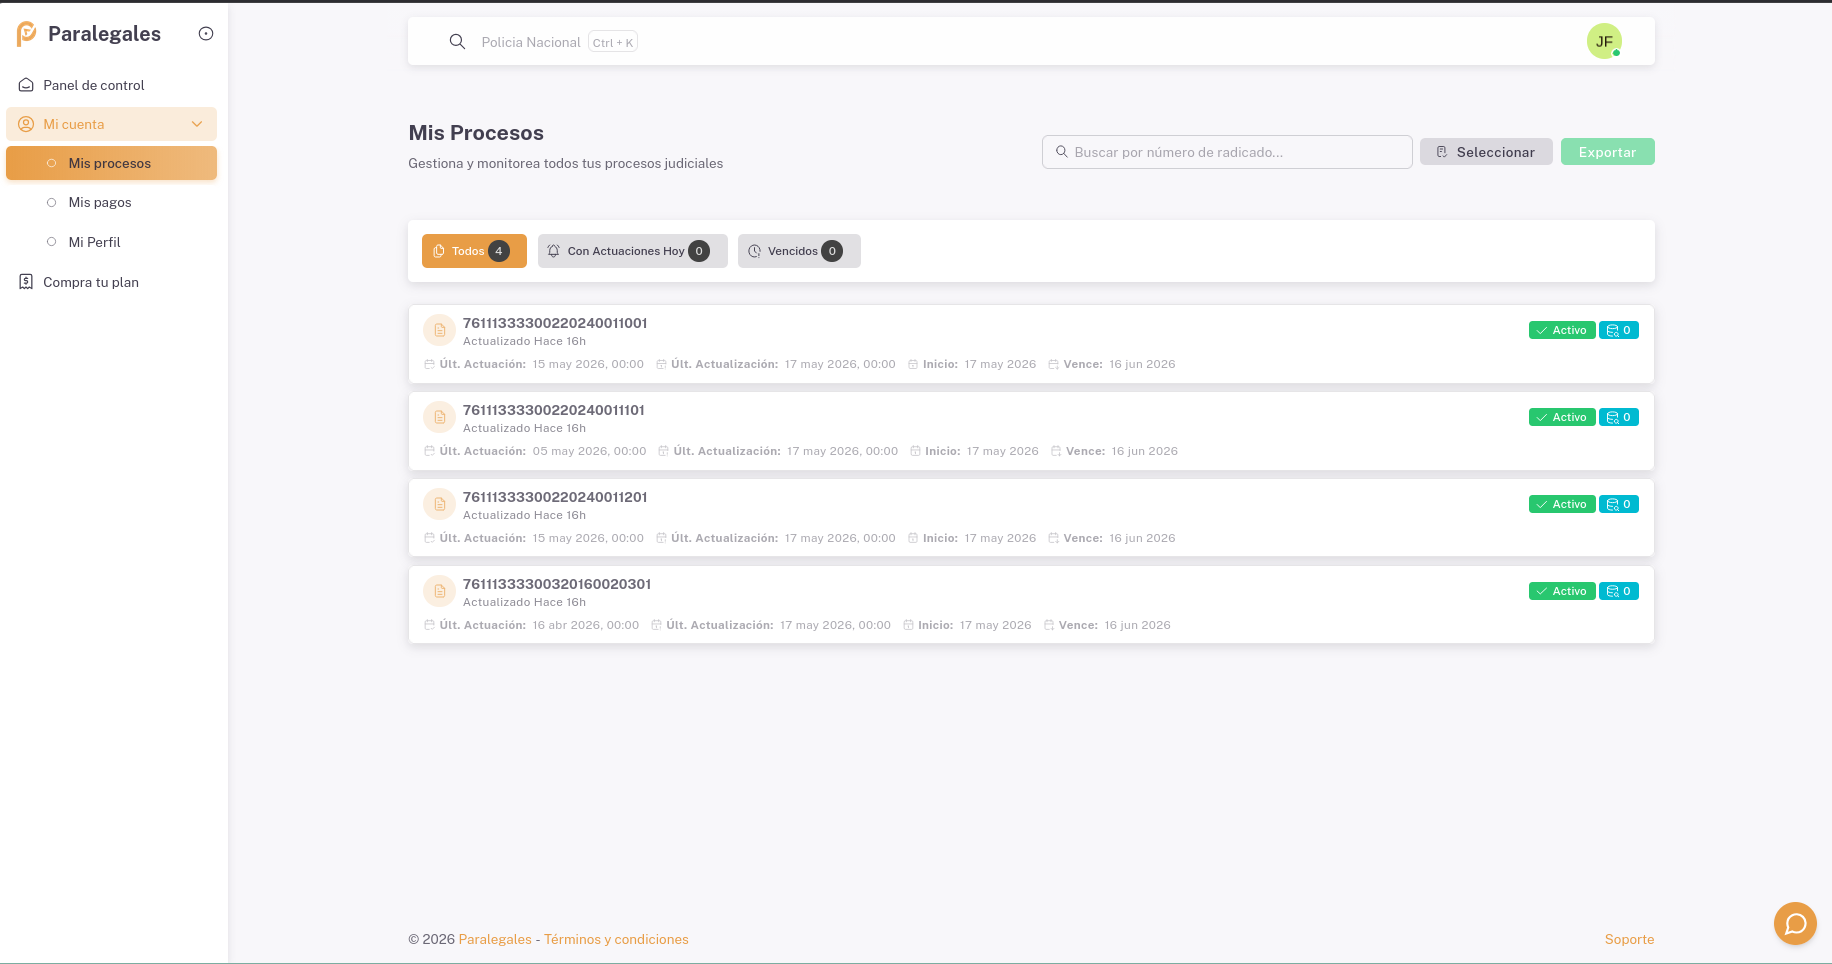
\includegraphics[width=1\textwidth]{img/figures/fig27-my-processes-view.png}
  \caption[\myProcessesViewCaption]{\myProcessesViewCaption Fuente: Elaboración propia.}
  \label{fig:my-processes-view}
\end{figure}

\subsubsection{Automatización mediante Seguimientos Activos}

Más allá del seguimiento manual, el módulo introduce un subsistema de automatización denominado ``Seguimientos Activos''. Esta funcionalidad exime al usuario de realizar consultas manuales repetitivas al delegar al sistema la búsqueda diaria de procesos judiciales asociados a un parámetro de interés, tal como un Número de Identificación Tributaria (NIT) o la Razón Social de una persona natural o jurídica.

A nivel arquitectónico en el \textit{frontend}, la lógica de negocio y las peticiones de red fueron abstraídas en funciones componibles (\textit{composables}), las cuales alimentan las interfaces de usuario de manera reactiva. La creación de un nuevo seguimiento requiere la validación y vinculación a un plan de pago o suscripción activa del usuario, integrando así los servicios operativos con el modelo de facturación. Una vez configurado, el motor de búsqueda rastrea diversas bases de datos en segundo plano, incluyendo la Rama Judicial y el sistema de información SAMAI. La \autoref{fig:seguimiento-activo} muestra el formulario de configuración de un nuevo seguimiento activo, donde el usuario define el parámetro de búsqueda y lo vincula a su plan vigente.

\newcommand\seguimientoActivoCaption{Formulario de configuración de un nuevo seguimiento activo con vinculación al plan de suscripción. \hspace{1em}}
\begin{figure}[H]
  \centering
  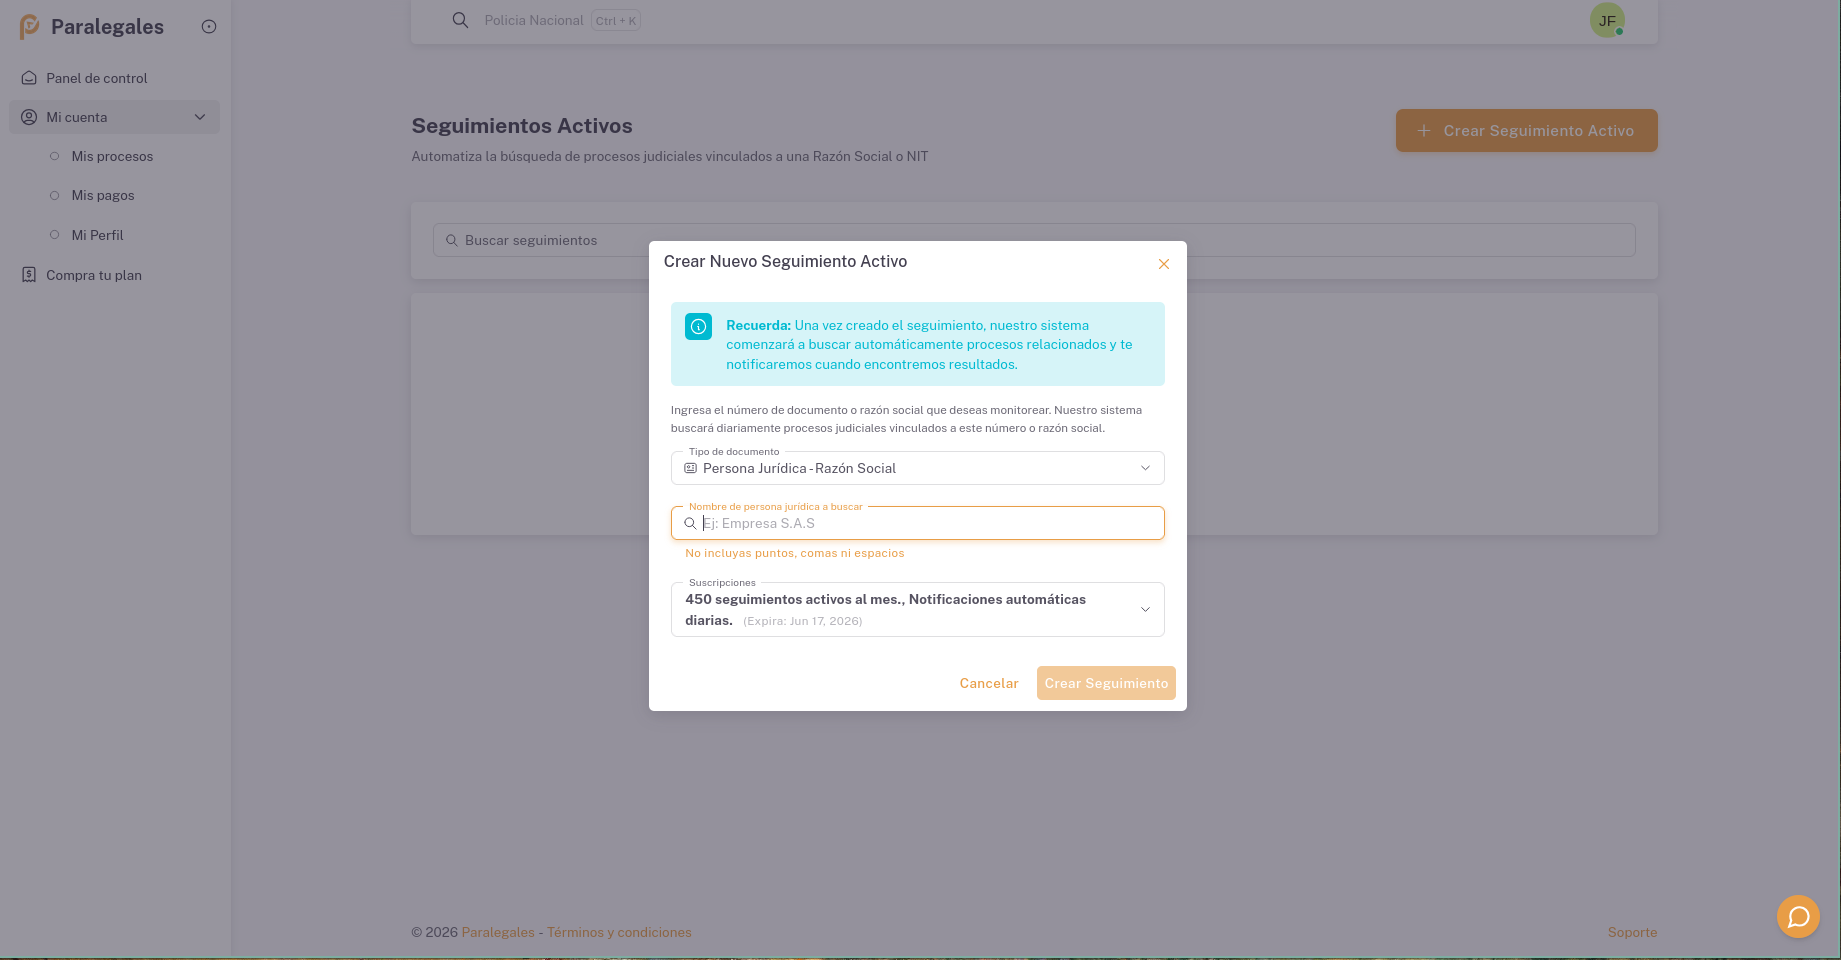
\includegraphics[width=1\textwidth]{img/figures/fig28-seguimiento-activo.png}
  \caption[\seguimientoActivoCaption]{\seguimientoActivoCaption Fuente: Elaboración propia.}
  \label{fig:seguimiento-activo}
\end{figure}

Para la revisión de los resultados, se diseñó una vista de detalle basada en pestañas que separa los ``Procesos Encontrados'' de una ``Lista Blanca''. Esta interfaz proporciona una experiencia de clasificación interactiva: el usuario puede revisar los nuevos hallazgos y decidir, mediante acciones asíncronas, si los aprueba (incorporándolos a su lista blanca) o los descarta (enviándolos a una lista negra). La \autoref{fig:seguimiento-activo-details} ilustra esta vista de detalle con los resultados organizados en pestañas, facilitando la clasificación progresiva de coincidencias. De esta manera, se garantiza un filtrado progresivo y personalizado, optimizando el tiempo invertido en la depuración de coincidencias homónimas o irrelevantes. La \autoref{fig:seguimiento-activo-success} confirma la retroalimentación visual que recibe el usuario al aprobar un proceso encontrado, reforzando la confianza en la operación completada.

\newcommand\seguimientoActivoDetailsCaption{Vista de detalle del seguimiento activo con resultados organizados en pestañas de clasificación. \hspace{1em}}
\begin{figure}[H]
  \centering
  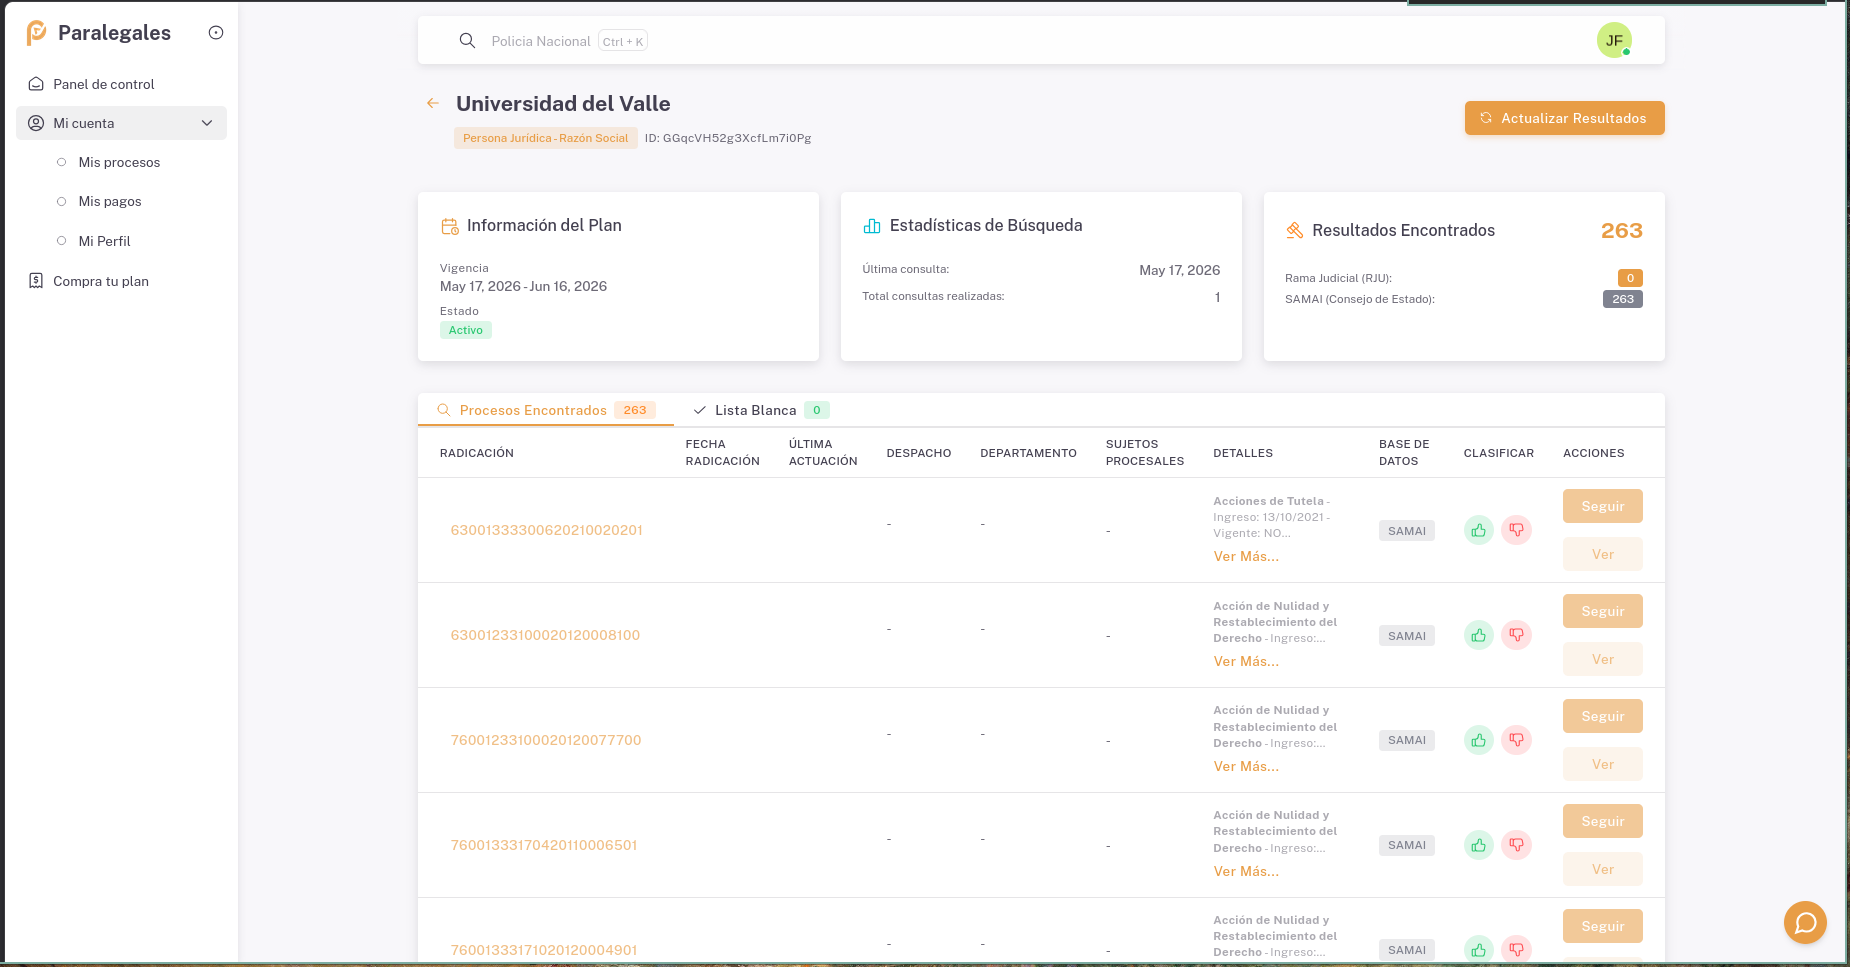
\includegraphics[width=1\textwidth]{img/figures/fig20-seguimiento-activo-details.png}
  \caption[\seguimientoActivoDetailsCaption]{\seguimientoActivoDetailsCaption Fuente: Elaboración propia.}
  \label{fig:seguimiento-activo-details}
\end{figure}

\newcommand\seguimientoActivoSuccessCaption{Confirmación visual tras la aprobación de un proceso encontrado en el seguimiento activo. \hspace{1em}}
\begin{figure}[H]
  \centering
  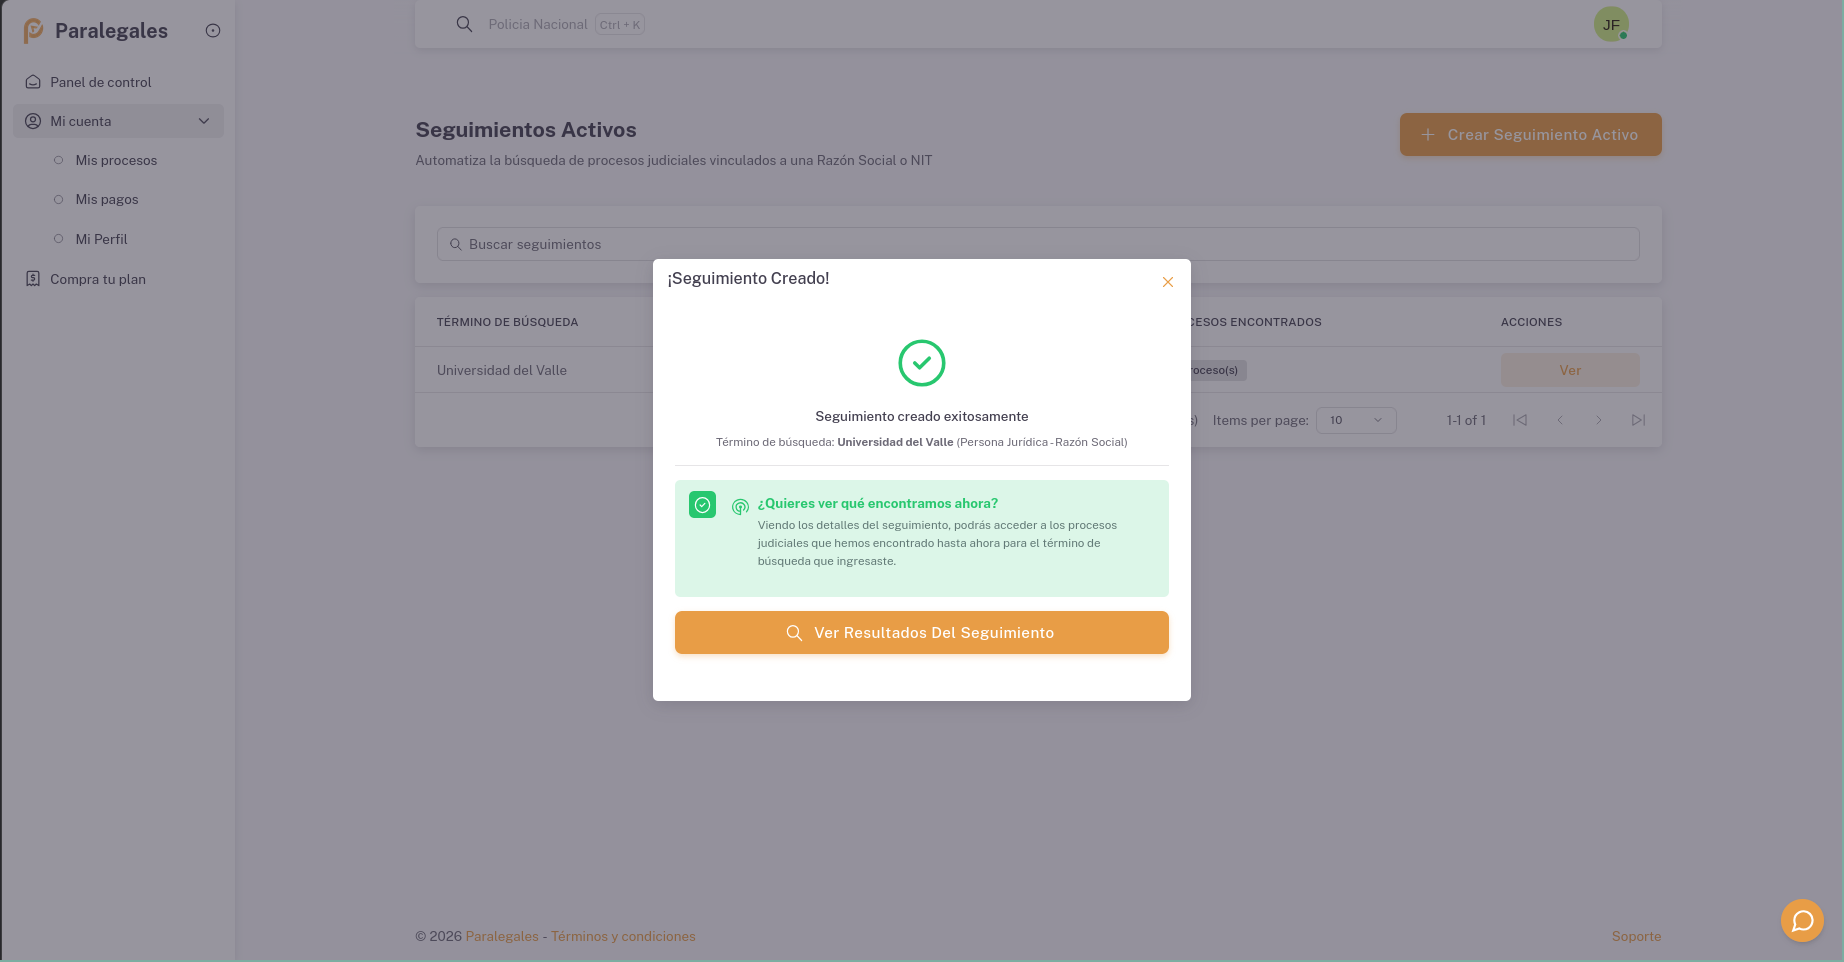
\includegraphics[width=1\textwidth]{img/figures/fig28-seguimiento-activo-success.png}
  \caption[\seguimientoActivoSuccessCaption]{\seguimientoActivoSuccessCaption Fuente: Elaboración propia.}
  \label{fig:seguimiento-activo-success}
\end{figure}

\subsubsection{Importación Masiva de Procesos}

Pensando en la usabilidad para nuevos despachos de abogados o equipos jurídicos con volúmenes considerables de casos, se implementó una funcionalidad de importación masiva que permite la carga simultánea de múltiples procesos en una sola operación.

Esta funcionalidad integra los módulos previamente descritos: recibe un conjunto de datos estructurado por parte del usuario y lo procesa de forma iterativa o por lotes en el \textit{backend}. El sistema verifica la existencia de cada proceso, valida los parámetros y ejecuta la lógica de seguimiento de forma individual, proporcionando al final un reporte sobre el estado de la importación. Esta operación optimiza drásticamente el tiempo operativo en comparación con el registro manual proceso por proceso, reduciendo la fricción inicial para equipos con carteras de casos de gran volumen. Complementando la operación orientada al usuario final, el siguiente módulo habilita la comunicación proactiva desde el portal administrativo, a través de campañas de mensajería masiva.
